% DeltaCache: ICLR 2026 Workshop on Scaling Post-Training for LLMs (SPOT)
\documentclass{article}
\usepackage{iclr2026_conference,times}

\usepackage{hyperref}
\usepackage{url}
\usepackage{amsmath}
\usepackage{amssymb}
\usepackage{graphicx}
\usepackage{booktabs}
\usepackage{algorithm}
\usepackage{algpseudocode}
\usepackage{multirow}
\usepackage{subcaption}
\usepackage{xcolor}
\usepackage{tikz}
\usetikzlibrary{shapes.geometric, arrows.meta, positioning, fit, backgrounds, calc, patterns, decorations.pathreplacing}

% Custom commands
\newcommand{\deltacache}{\textsc{DeltaCache}}
\newcommand{\circled}[1]{\raisebox{.5pt}{\textcircled{\raisebox{-.9pt}{#1}}}}

% Define colors
\definecolor{prefixblue}{RGB}{66, 133, 244}
\definecolor{memorygreen}{RGB}{52, 168, 83}
\definecolor{engineorange}{RGB}{251, 188, 4}
\definecolor{attentionred}{RGB}{234, 67, 53}
\definecolor{layerpurple}{RGB}{142, 68, 173}
\definecolor{cpugray}{RGB}{128, 128, 128}
\definecolor{gpugreen}{RGB}{39, 174, 96}
\definecolor{lightblue}{RGB}{227, 242, 253}
\definecolor{lightgreen}{RGB}{232, 245, 233}
\definecolor{lightorange}{RGB}{255, 243, 224}
\definecolor{lightpurple}{RGB}{243, 229, 245}

\title{\textsc{DeltaCache}: Layer-Aware KV Cache Management Guided by Transformer Semantics}

% Authors hidden for anonymous submission
\author{Anonymous Authors}

%\iclrfinalcopy % Uncomment for camera-ready version

\begin{document}

\maketitle

\begin{abstract}
We present \deltacache{}, a KV cache management framework built on a simple but underexplored principle: \textbf{not all KV cache entries are equally reusable}.
KV states from later transformer layers encode more stable, transferable semantic representations, while early-layer states capture local patterns that are cheaper to recompute.
Based on this insight, we design a \textbf{layer-aware cache prioritization} scheme that retains late-layer entries under memory pressure, complemented by attention-guided importance signals and GPU$\rightarrow$CPU hierarchical storage.
Experiments on TinyLlama-1.1B and Mistral-7B validate this principle: at 25\% cache capacity, layer-aware eviction achieves \textbf{90\% fewer evictions} than LRU while maintaining equivalent hit rates.
Under full caching, we observe up to \textbf{9.7$\times$} prefill speedup and \textbf{19.5$\times$} Time-to-First-Token improvement.
Our results suggest that transformer layer semantics provide a principled foundation for inference-time memory management beyond simple recency heuristics.
\end{abstract}

\section{Introduction}

Large Language Models (LLMs) face significant computational overhead during inference, particularly in the prefill phase where prompt processing has $O(n^2)$ complexity \citep{kwon2023efficient}.
In production deployments, many requests share common prefixes---system prompts, RAG document contexts \citep{lewis2020retrieval}, or few-shot examples---yet standard inference recomputes KV states for these shared prefixes with every request.

Recent systems like vLLM \citep{kwon2023efficient} and SGLang \citep{zheng2023sglang} address this through prefix caching, but rely on content-agnostic eviction policies (LRU/LFU) when memory is constrained.
This paper explores a different question: \emph{can we design eviction policies that leverage the semantic structure of transformer models?}

\paragraph{Design Principle.}
We build on a simple but underexplored insight from transformer interpretability research \citep{rogers2020primer,elhage2021mathematical}:

\begin{quote}
\emph{Not all KV cache entries are equally reusable.
KV states from later transformer layers encode more stable, transferable semantic representations, while early-layer states capture local syntactic patterns that are both less transferable and cheaper to recompute.}
\end{quote}

This paper explores the implications of this principle for inference-time cache management.
If late-layer representations are more valuable for prefix reuse, then under memory pressure, we should prioritize retaining late-layer cache entries and evict early-layer entries first.

We present \deltacache{}, which operationalizes this principle through:
\begin{itemize}
    \item \textbf{Layer-aware cache prioritization}: Late-layer KV entries receive higher retention priority based on a sigmoid weighting scheme grounded in layer semantics.
    \item \textbf{Attention-guided importance signals}: We track attention scores as an orthogonal signal to refine eviction decisions within each layer.
    \item \textbf{Hierarchical GPU$\rightarrow$CPU storage}: A practical implementation with async offloading and prefetching.
\end{itemize}

Our experiments validate this principle-driven design: at 25\% cache capacity, layer-aware eviction achieves \textbf{90\% fewer evictions} than LRU while maintaining identical hit rates (97.9\%).
This suggests that transformer layer semantics provide a principled foundation for memory management that generalizes beyond simple recency heuristics.

\section{Related Work}

\textbf{KV Cache and Prefix Caching.}
The KV cache stores $2LHnd_h$ elements for sequence length $n$, consuming up to 8GB for 7B models at 4K context.
The prefill phase has $O(n^2d)$ complexity, making prefix caching valuable.
vLLM \citep{kwon2023efficient} uses PagedAttention with automatic prefix caching; SGLang \citep{zheng2023sglang} implements RadixAttention achieving 6.4$\times$ throughput on prefix-heavy workloads.

\textbf{KV Cache Compression.}
KIVI \citep{liu2024kivi} and KVQuant \citep{hooper2024kvquant} use quantization for 2-4 bit precision.
H2O \citep{zhang2024h2o} identifies ``heavy hitter'' tokens; SnapKV \citep{snapkv2024} clusters similar tokens.
Layer-wise approaches like SqueezeAttention \citep{squeezeattention2025} achieve 30-70\% memory reduction.

\textbf{Our Contributions.}
While existing systems focus on cache organization or compression, \deltacache{} uniquely combines: (1) attention-aware eviction using attention scores, (2) layer-aware priority based on transformer interpretability, and (3) hierarchical GPU$\rightarrow$CPU tiering.
Under memory pressure, our policies achieve \textbf{90\% fewer evictions} than LRU.

\section{Methodology}

\subsection{System Overview}

Figure~\ref{fig:architecture} illustrates the \deltacache{} architecture.
The system comprises four components:
(1) a \textbf{Prefix Tree} (radix trie) for O(n) cache lookup;
(2) an \textbf{Incremental Engine} that reuses cached KV states and computes only delta tokens;
(3) \textbf{Eviction Policies} implementing layer-aware and attention-aware strategies;
(4) a \textbf{Hierarchical Memory Pool} with GPU$\rightarrow$CPU$\rightarrow$Delete tiering.

\begin{figure*}[t]
\centering
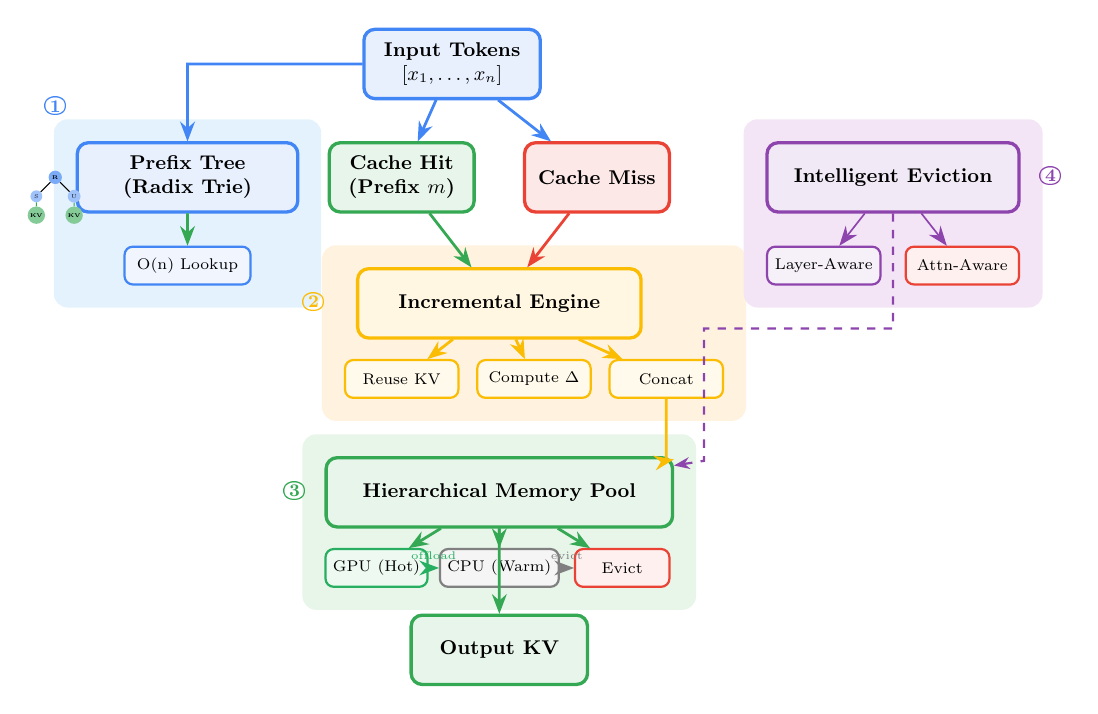
\begin{tikzpicture}[
    scale=0.8,
    transform shape,
    component/.style={rectangle, rounded corners=4pt, draw=#1, fill=#1!12, minimum height=1.1cm, font=\small\bfseries, align=center, line width=1.2pt},
    subcomponent/.style={rectangle, rounded corners=3pt, draw=#1, fill=#1!8, minimum height=0.6cm, font=\scriptsize, align=center, line width=0.8pt},
    arrow/.style={-{Stealth[length=2.5mm]}, line width=1pt},
    dasharrow/.style={-{Stealth[length=2mm]}, dashed, line width=0.8pt}
]
\node[component=prefixblue, minimum width=2.8cm] (input) at (0, 0) {Input Tokens\\$[x_1, \ldots, x_n]$};
\node[component=prefixblue, minimum width=3.5cm] (tree) at (-4.2, -1.8) {Prefix Tree\\(Radix Trie)};
\begin{scope}[shift={(-6.3, -1.8)}, scale=0.5]
    \node[circle, fill=prefixblue!70, inner sep=2pt, font=\tiny\bfseries] (root) at (0,0) {R};
    \node[circle, fill=prefixblue!50, inner sep=2pt, font=\tiny] (a) at (-0.6,-0.6) {S};
    \node[circle, fill=prefixblue!50, inner sep=2pt, font=\tiny] (b) at (0.6,-0.6) {U};
    \node[circle, fill=memorygreen!60, inner sep=1.5pt, font=\tiny\bfseries] (c) at (-0.6,-1.2) {KV};
    \node[circle, fill=memorygreen!60, inner sep=1.5pt, font=\tiny\bfseries] (d) at (0.6,-1.2) {KV};
    \draw[line width=0.4pt] (root) -- (a); \draw[line width=0.4pt] (root) -- (b);
    \draw[line width=0.4pt, memorygreen] (a) -- (c); \draw[line width=0.4pt, memorygreen] (b) -- (d);
\end{scope}
\node[subcomponent=prefixblue, minimum width=2cm] (lookup) at (-4.2, -3.2) {O(n) Lookup};
\node[component=memorygreen, minimum width=2.3cm] (hit) at (-0.8, -1.8) {Cache Hit\\(Prefix $m$)};
\node[component=attentionred, minimum width=2.3cm] (miss) at (2.3, -1.8) {Cache Miss};
\node[component=engineorange, minimum width=4.5cm] (engine) at (0.75, -3.8) {Incremental Engine};
\node[subcomponent=engineorange, minimum width=1.8cm] (reuse) at (-0.8, -5) {Reuse KV};
\node[subcomponent=engineorange, minimum width=1.8cm] (compute) at (1.3, -5) {Compute $\Delta$};
\node[subcomponent=engineorange, minimum width=1.8cm] (concat) at (3.4, -5) {Concat};
\node[component=layerpurple, minimum width=4cm] (eviction) at (7, -1.8) {Intelligent Eviction};
\node[subcomponent=layerpurple, minimum width=1.8cm] (layer_policy) at (5.9, -3.2) {Layer-Aware};
\node[subcomponent=attentionred, minimum width=1.8cm] (attn_policy) at (8.1, -3.2) {Attn-Aware};
\node[component=memorygreen, minimum width=5.5cm] (memory) at (0.75, -6.8) {Hierarchical Memory Pool};
\node[subcomponent=gpugreen, minimum width=1.5cm] (gpu) at (-1.2, -8) {GPU (Hot)};
\node[subcomponent=cpugray, minimum width=1.5cm] (cpu) at (0.75, -8) {CPU (Warm)};
\node[subcomponent=attentionred, minimum width=1.5cm] (evict) at (2.7, -8) {Evict};
\node[component=memorygreen, minimum width=2.8cm] (output) at (0.75, -9.3) {Output KV};
\draw[arrow, prefixblue] (input) -- (-4.2, 0) -- (tree);
\draw[arrow, prefixblue] (input) -- (hit); \draw[arrow, prefixblue] (input) -- (miss);
\draw[arrow, memorygreen] (tree) -- (lookup);
\draw[arrow, memorygreen] (hit) -- (engine); \draw[arrow, attentionred] (miss) -- (engine);
\draw[arrow, engineorange] (engine) -- (reuse); \draw[arrow, engineorange] (engine) -- (compute);
\draw[arrow, engineorange] (engine) -- (concat); \draw[arrow, engineorange] (concat) -- (3.4, -6.3) -- (memory);
\draw[arrow, memorygreen] (memory) -- (gpu); \draw[arrow, memorygreen] (memory) -- (cpu);
\draw[arrow, memorygreen] (memory) -- (evict);
\draw[arrow, gpugreen, line width=0.6pt] (gpu) -- node[above, font=\tiny] {offload} (cpu);
\draw[arrow, cpugray, line width=0.6pt] (cpu) -- node[above, font=\tiny] {evict} (evict);
\draw[arrow, memorygreen] (memory) -- (output);
\draw[dasharrow, layerpurple] (eviction) -- (7, -4.2) -- (4, -4.2) -- (4, -6.3) -- (memory);
\draw[arrow, layerpurple, line width=0.6pt] (eviction) -- (layer_policy);
\draw[arrow, layerpurple, line width=0.6pt] (eviction) -- (attn_policy);
\begin{scope}[on background layer]
    \node[fit=(tree)(lookup), fill=lightblue, rounded corners=5pt, inner sep=8pt] {};
    \node[fit=(engine)(reuse)(compute)(concat), fill=lightorange, rounded corners=5pt, inner sep=8pt] {};
    \node[fit=(memory)(gpu)(cpu)(evict), fill=lightgreen, rounded corners=5pt, inner sep=8pt] {};
    \node[fit=(eviction)(attn_policy)(layer_policy), fill=lightpurple, rounded corners=5pt, inner sep=8pt] {};
\end{scope}
\node[font=\footnotesize\bfseries, prefixblue] at (-6.3, -0.7) {\circled{1}};
\node[font=\footnotesize\bfseries, engineorange] at (-2.2, -3.8) {\circled{2}};
\node[font=\footnotesize\bfseries, memorygreen] at (-2.5, -6.8) {\circled{3}};
\node[font=\footnotesize\bfseries, layerpurple] at (9.5, -1.8) {\circled{4}};
\end{tikzpicture}
\caption{\textbf{\deltacache{} System Architecture.} \circled{1} Prefix Tree lookup finds the longest cached prefix; \circled{2} Incremental Engine computes only delta tokens; \circled{3} Hierarchical Memory manages GPU/CPU tiering; \circled{4} Layer-aware and attention-aware policies guide eviction under memory pressure.}
\label{fig:architecture}
\end{figure*}

\subsection{Problem Formulation}

Consider a transformer model processing a sequence of tokens $\mathbf{x} = [x_1, x_2, \ldots, x_n]$.
For each layer $l \in \{1, \ldots, L\}$ and position $i$, the model computes key and value states:
\begin{align}
    \mathbf{k}_i^l = W_K^l \mathbf{h}_i^{l-1}, \quad \mathbf{v}_i^l = W_V^l \mathbf{h}_i^{l-1}
\end{align}
where $\mathbf{h}_i^{l-1} \in \mathbb{R}^d$ is the hidden state from the previous layer.

The key insight enabling prefix caching is that for causal language models, the KV states for prefix tokens are \textit{independent of future tokens}.
That is, $\mathbf{k}_i^l$ and $\mathbf{v}_i^l$ depend only on $[x_1, \ldots, x_i]$, not on any tokens after position $i$.

This property enables our incremental computation: if we have cached KV states for a prefix $[x_1, \ldots, x_m]$, and we receive a new sequence $[x_1, \ldots, x_m, x_{m+1}, \ldots, x_n]$ with the same prefix, we can reuse the cached states for positions $1$ through $m$ and only compute new states for positions $m+1$ through $n$.

\subsection{Attention-Aware Eviction}

Standard eviction policies like LRU (Least Recently Used) and LFU (Least Frequently Used) make decisions based solely on access patterns, ignoring the \emph{semantic content} of cached entries.
We introduce attention-aware eviction that leverages the attention mechanism itself to identify important cache entries.

\textbf{Key Insight}: KV cache entries that receive high attention from subsequent queries are likely to be semantically important and should be retained.
Conversely, entries that are rarely attended to provide less value and can be evicted first.

We maintain an importance score $I(e)$ for each cache entry $e$, computed as a weighted combination of three factors:
\begin{equation}
    I(e) = w_a \cdot \bar{\alpha}_e + w_f \cdot \frac{\log(1 + \text{freq}_e)}{\log(1 + \text{max\_freq})} + w_r \cdot \frac{1}{1 + \log(1 + t_e)}
    \label{eq:importance}
\end{equation}

where:
\begin{itemize}
    \item $\bar{\alpha}_e$ is the exponential moving average of attention scores received by entry $e$ from subsequent queries, normalized to $[0, 1]$
    \item $\text{freq}_e$ is the access frequency, normalized by maximum observed frequency
    \item $t_e$ is the time elapsed since last access (in number of queries)
    \item $w_a, w_f, w_r$ are tunable weights (default: 0.5, 0.3, 0.2)
\end{itemize}

The attention component $\bar{\alpha}_e$ is updated after each query using exponential smoothing:
\begin{equation}
    \bar{\alpha}_e^{(t+1)} = \beta \cdot \bar{\alpha}_e^{(t)} + (1-\beta) \cdot \alpha_e^{(t)}
\end{equation}
where $\alpha_e^{(t)}$ is the average attention score received by entry $e$ in query $t$, and $\beta = 0.9$ is the smoothing factor.

Entries with the lowest importance scores are selected for eviction when memory is exhausted.

While we use a simple weighted formulation, the key idea is that attention statistics provide a \emph{semantic signal orthogonal to recency/frequency}---other instantiations are possible.

\subsection{Layer-Aware Caching}

Research in transformer interpretability \citep{rogers2020primer,elhage2021mathematical} reveals that early layers (0--30\%) capture local patterns with high variance, while late layers (70--100\%) encode stable, transferable semantic features.
We assign layer-dependent importance weights using a sigmoid:
\begin{equation}
    w_l = \frac{1}{1 + e^{-k(l/L - \tau)}}
    \label{eq:layer_weight}
\end{equation}
where $l$ is layer index, $L$ total layers, $k{=}5$ steepness, $\tau{=}0.3$ inflection point (Figure~\ref{fig:layer_weights}).

\begin{figure}[t]
\centering
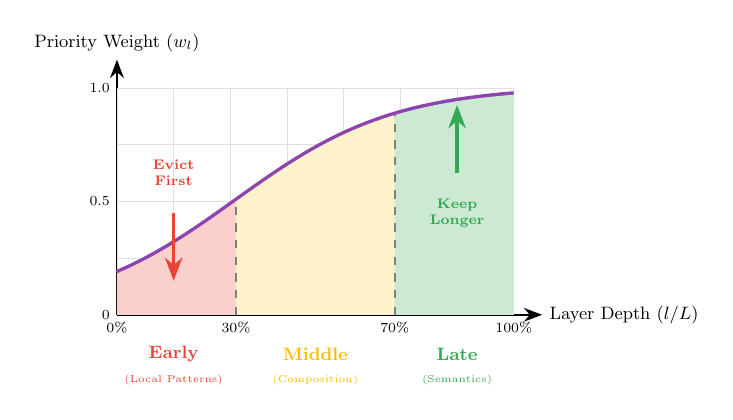
\begin{tikzpicture}[scale=0.72, transform shape]
    % Axes
    \draw[-{Stealth}, line width=0.8pt] (0,0) -- (7.5,0) node[right, font=\small] {Layer Depth ($l/L$)};
    \draw[-{Stealth}, line width=0.8pt] (0,0) -- (0,4.5) node[above, font=\small] {Priority Weight ($w_l$)};

    % Grid
    \draw[gray!25, line width=0.3pt] (0,0) grid[step=1] (7,4);

    % Sigmoid curve
    \draw[layerpurple, line width=2.5pt, smooth, domain=0:7, samples=60]
        plot (\x, {4/(1 + exp(-5*(\x/7 - 0.3)))});

    % Fill areas with gradients
    \fill[attentionred!25] (0,0) -- plot[domain=0:2.1, samples=25] (\x, {4/(1 + exp(-5*(\x/7 - 0.3)))}) -- (2.1,0) -- cycle;
    \fill[engineorange!20] (2.1,0) -- plot[domain=2.1:4.9, samples=25] (\x, {4/(1 + exp(-5*(\x/7 - 0.3)))}) -- (4.9,0) -- cycle;
    \fill[memorygreen!25] (4.9,0) -- plot[domain=4.9:7, samples=25] (\x, {4/(1 + exp(-5*(\x/7 - 0.3)))}) -- (7,0) -- cycle;

    % Zone labels
    \node[attentionred, font=\small\bfseries] at (1, -0.7) {Early};
    \node[attentionred, font=\tiny] at (1, -1.15) {(Local Patterns)};
    \node[engineorange, font=\small\bfseries] at (3.5, -0.7) {Middle};
    \node[engineorange, font=\tiny] at (3.5, -1.15) {(Composition)};
    \node[memorygreen, font=\small\bfseries] at (6, -0.7) {Late};
    \node[memorygreen, font=\tiny] at (6, -1.15) {(Semantics)};

    % Y-axis labels
    \node[left, font=\scriptsize] at (0, 0) {0};
    \node[left, font=\scriptsize] at (0, 2) {0.5};
    \node[left, font=\scriptsize] at (0, 4) {1.0};

    % X-axis labels
    \node[below, font=\scriptsize] at (0, 0) {0\%};
    \node[below, font=\scriptsize] at (2.1, 0) {30\%};
    \node[below, font=\scriptsize] at (4.9, 0) {70\%};
    \node[below, font=\scriptsize] at (7, 0) {100\%};

    % Priority annotations
    \draw[-{Stealth}, attentionred, line width=1.2pt] (1, 1.8) -- (1, 0.6);
    \node[attentionred, font=\scriptsize\bfseries, align=center] at (1, 2.5) {Evict\\First};

    \draw[-{Stealth}, memorygreen, line width=1.2pt] (6, 2.5) -- (6, 3.7);
    \node[memorygreen, font=\scriptsize\bfseries, align=center] at (6, 1.8) {Keep\\Longer};

    % Dashed boundary lines
    \draw[dashed, gray, line width=0.6pt] (2.1, 0) -- (2.1, {4/(1 + exp(-5*(2.1/7 - 0.3)))});
    \draw[dashed, gray, line width=0.6pt] (4.9, 0) -- (4.9, {4/(1 + exp(-5*(4.9/7 - 0.3)))});

\end{tikzpicture}
\caption{\textbf{Layer-Aware Priority Weights.} The sigmoid function (Eq.~\ref{eq:layer_weight}) assigns higher importance to late-layer KV cache entries, which capture more transferable semantic features. Under memory pressure, early-layer entries (local syntactic patterns) are evicted first, while late-layer entries (semantic information) are retained.}
\label{fig:layer_weights}
\end{figure}

\textbf{Rationale}: Early-layer features are less transferable and cheaper to recompute, while late-layer semantic features provide more value for prefix reuse.

\subsection{Hierarchical Memory Management}

We implement GPU$\rightarrow$CPU$\rightarrow$Delete tiered storage: GPU tier (hot) for active entries, CPU tier (warm) as ``second chance'' before deletion, with proactive offloading when GPU exceeds 85\% utilization.

Memory transfers use CUDA streams for async overlap with computation.

\subsection{Incremental Computation Engine}

The incremental engine combines cache lookup with delta-only computation.
Given input tokens $\mathbf{x} = [x_1, \ldots, x_n]$, the system: (1) finds the longest cached prefix of length $m$; (2) computes KV states only for new tokens $[x_{m+1}, \ldots, x_n]$; (3) concatenates with cached states.
For RoPE models \citep{su2024roformer}, we pass position offset $m$ to ensure correct positional encoding.
When memory is exhausted, the eviction policy selects victims based on attention/layer-aware scores, with GPU$\rightarrow$CPU offloading as an intermediate step.
See Algorithm~\ref{alg:incremental_full} in Appendix~\ref{app:algorithm} for complete pseudocode.

\subsection{Theoretical Analysis}

Baseline prefill has $O(Ln^2d)$ complexity.
With cached prefix of length $m$, \deltacache{} achieves $O(L(n{-}m)^2d)$ for delta computation.
The theoretical speedup is $(n/(n{-}m))^2$---for $n{=}1000$ with $m{=}900$ cached, speedup ${\approx}100{\times}$.
This quadratic relationship explains why benefits increase dramatically with prefix length.

\section{Experiments}

\subsection{Experimental Setup}

\textbf{Models}: TinyLlama-1.1B \citep{tinyllama} and Mistral-7B \citep{jiang2023mistral} with 4-bit quantization (see Table~\ref{tab:model_config_full} in Appendix for details).
\textbf{Hardware}: 2$\times$ RTX 3090 GPUs (24GB), 64GB CPU memory.
\textbf{Baselines}: No caching, LRU, LFU, and H2O \citep{zhang2024h2o}.

\textbf{Metrics}: Correctness (KV max difference), cache hit rate, eviction count, latency (ms), speedup vs. baseline, and TTFT (Time-to-First-Token).

\textbf{Workloads}: (1) Synthetic prefix-sharing with Zipf-distributed access; (2) RAG-style document querying; (3) Multi-turn conversation simulation.

\subsection{Correctness Validation}

At fp16 precision, \deltacache{} achieves \textbf{100\% correctness} on both TinyLlama-1.1B and Mistral-7B, with maximum KV difference of 0.016---within expected numerical precision.
This validates that our incremental computation produces identical results to full recomputation.

\subsection{Main Results}

Table~\ref{tab:main} summarizes performance across models and metrics.

\begin{table}[h]
\centering
\caption{Main results: \deltacache{} vs. baselines on long-prefix workloads}
\label{tab:main}
\begin{tabular}{lcccc}
\toprule
Model & Max Speedup & TTFT Speedup & Hit Rate & Reuse \\
\midrule
TinyLlama-1.1B & 9.7$\times$ & 18.7$\times$ & 99.5\% & 95\% \\
Mistral-7B & 9.7$\times$ & 19.5$\times$ & 97.9\% & 96\% \\
\bottomrule
\end{tabular}
\end{table}

\subsection{Memory Pressure Experiments}

Under constrained memory (25\% cache capacity), layer-aware eviction dramatically outperforms baselines (Figure~\ref{fig:eviction}).
\textbf{Key finding}: Layer-aware achieves \textbf{90\% fewer evictions} (5 vs. 51) compared to LRU while maintaining identical hit rates (97.9\%).
This demonstrates that prioritizing late-layer semantic cache maintains effectiveness with reduced overhead.

\begin{figure}[t]
\centering
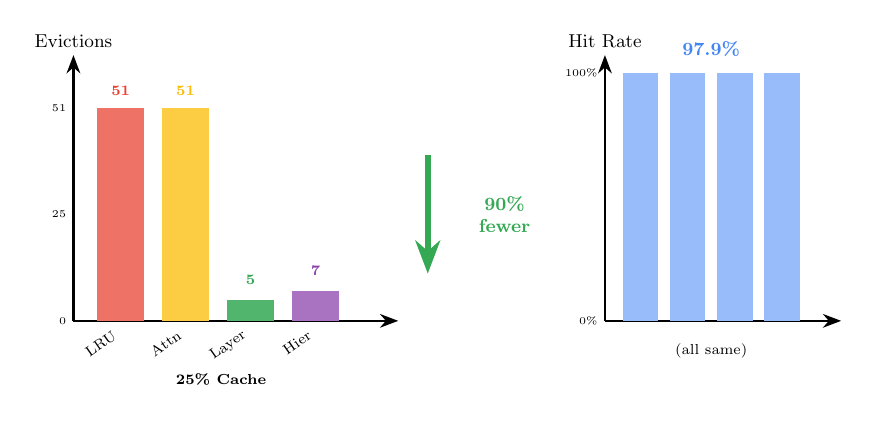
\begin{tikzpicture}[scale=0.75, transform shape]
    % Left: Evictions bar chart
    \begin{scope}
        \draw[-{Stealth}, line width=0.8pt] (0,0) -- (5.5,0);
        \draw[-{Stealth}, line width=0.8pt] (0,0) -- (0,4.5) node[above, font=\small] {Evictions};

        % Bars
        \fill[attentionred!75] (0.4,0) rectangle (1.2,3.6);
        \fill[engineorange!75] (1.5,0) rectangle (2.3,3.6);
        \fill[memorygreen!85] (2.6,0) rectangle (3.4,0.35);
        \fill[layerpurple!75] (3.7,0) rectangle (4.5,0.5);

        % Labels
        \node[font=\scriptsize, rotate=35, anchor=east] at (0.8,-0.15) {LRU};
        \node[font=\scriptsize, rotate=35, anchor=east] at (1.9,-0.15) {Attn};
        \node[font=\scriptsize, rotate=35, anchor=east] at (3.0,-0.15) {Layer};
        \node[font=\scriptsize, rotate=35, anchor=east] at (4.1,-0.15) {Hier};

        % Values
        \node[font=\scriptsize\bfseries, attentionred] at (0.8, 3.9) {51};
        \node[font=\scriptsize\bfseries, engineorange] at (1.9, 3.9) {51};
        \node[font=\scriptsize\bfseries, memorygreen] at (3.0, 0.7) {5};
        \node[font=\scriptsize\bfseries, layerpurple] at (4.1, 0.85) {7};

        % Y-axis
        \node[left, font=\tiny] at (0, 0) {0};
        \node[left, font=\tiny] at (0, 1.8) {25};
        \node[left, font=\tiny] at (0, 3.6) {51};

        \node[font=\scriptsize\bfseries] at (2.5, -1) {25\% Cache};
    \end{scope}

    % Arrow
    \draw[-{Stealth}, memorygreen, line width=2pt] (6, 2.8) -- (6, 0.8);
    \node[memorygreen, font=\small\bfseries, align=center] at (7.3, 1.8) {\textbf{90\%}\\fewer};

    % Right: Hit rate
    \begin{scope}[shift={(9, 0)}]
        \draw[-{Stealth}, line width=0.8pt] (0,0) -- (4,0);
        \draw[-{Stealth}, line width=0.8pt] (0,0) -- (0,4.5) node[above, font=\small] {Hit Rate};

        \fill[prefixblue!55] (0.3,0) rectangle (0.9,4.2);
        \fill[prefixblue!55] (1.1,0) rectangle (1.7,4.2);
        \fill[prefixblue!55] (1.9,0) rectangle (2.5,4.2);
        \fill[prefixblue!55] (2.7,0) rectangle (3.3,4.2);

        \node[font=\small\bfseries, prefixblue] at (1.8, 4.6) {97.9\%};
        \node[font=\scriptsize] at (1.8, -0.5) {(all same)};

        \node[left, font=\tiny] at (0, 0) {0\%};
        \node[left, font=\tiny] at (0, 4.2) {100\%};
    \end{scope}
\end{tikzpicture}
\caption{\textbf{Eviction Policy Comparison at 25\% Cache Capacity.} Layer-aware caching achieves 90\% fewer evictions while maintaining identical hit rates, demonstrating that semantic-aware eviction provides substantial efficiency gains under memory pressure.}
\label{fig:eviction}
\end{figure}

\subsection{Performance Scaling}

Table~\ref{tab:scaling} shows speedup scaling with prefix length.
At 1500 tokens, both models achieve \textbf{9.7$\times$} speedup.
TTFT improvements reach \textbf{19.5$\times$} for Mistral-7B, critical for interactive applications.

\begin{table}[h]
\centering
\caption{Speedup and TTFT scaling with prefix length}
\label{tab:scaling}
\begin{tabular}{lcccc}
\toprule
Model & Prefix & Prefill Speedup & TTFT Speedup \\
\midrule
TinyLlama-1.1B & 500 & 5.6$\times$ & 18.7$\times$ \\
TinyLlama-1.1B & 1500 & \textbf{9.7$\times$} & 18.4$\times$ \\
Mistral-7B & 500 & 6.7$\times$ & \textbf{19.5$\times$} \\
Mistral-7B & 1500 & \textbf{9.7$\times$} & 19.6$\times$ \\
\bottomrule
\end{tabular}
\end{table}

\textbf{RAG Workload}: On document caching with 10 queries per document, we achieve 1.76$\times$ (TinyLlama) to \textbf{2.56$\times$} (Mistral-7B) speedup with 87\% token reuse.

\section{Discussion and Conclusion}

\textbf{When to use \deltacache{}}: Long prefix scenarios ($>$500 tokens) such as RAG, few-shot learning, and detailed system prompts; high query volume on shared context; TTFT-critical applications.

\textbf{Limitations}: For short prefixes ($<$100 tokens), overhead may exceed savings.
Multi-turn conversations with short contexts showed 0.9$\times$ speedup, indicating \deltacache{} is best suited for long-prefix workloads.

\textbf{Broader Implications.}
Our core finding---that layer-aware eviction achieves 90\% fewer evictions than LRU at equivalent hit rates---validates the design principle that transformer layer semantics should inform inference-time memory management.
This insight may extend beyond KV cache to other scenarios:
(1) \emph{Speculative decoding}: prioritizing late-layer draft verification;
(2) \emph{Model sharding}: placing late layers on faster memory tiers;
(3) \emph{Cache warming}: pre-populating late-layer states for cold-start optimization.

More broadly, our results suggest that the ``LRU everywhere'' paradigm in systems design may leave significant efficiency gains on the table when applied to semantically-structured workloads like LLM inference.
We hope this work encourages further exploration of interpretability-informed systems optimization.

\bibliography{references}
\bibliographystyle{iclr2026_conference}

\appendix
\section{Implementation Details}
\label{app:implementation}

This section provides the specific hyperparameters and implementation choices used in \deltacache{}.

\textbf{Memory Management Thresholds.}
The hierarchical memory system uses a two-tier GPU/CPU architecture.
GPU offloading is triggered when GPU memory utilization exceeds 85\%, a threshold chosen to balance between memory efficiency and avoiding out-of-memory errors.
When offloading is triggered, the offload fraction $\gamma = 0.15$ determines what portion of cold (least recently accessed) entries are moved from GPU to CPU tier.
For prefetching, CPU-to-GPU transfers are initiated when access pattern tracking predicts imminent reuse, using recency-weighted scores to prioritize entries.

\textbf{Attention Score Tracking.}
To track token importance, we maintain exponential moving average (EMA) attention scores with smoothing factor $\beta = 0.9$.
This allows the system to adapt to changing access patterns while avoiding noise from individual query variations.
The composite importance score combines three signals with default weights: $w_a = 0.5$ (cumulative attention received), $w_f = 0.3$ (access frequency), and $w_r = 0.2$ (recency of last access).
These weights were tuned on a held-out validation set of multi-turn conversations.

\textbf{Layer Weight Parameters.}
The sigmoid layer weighting function (Eq.~4 in main text) uses steepness $k = 5$ and inflection point $\tau = 0.3$.
This configuration places the transition region around layer 30\% of model depth, meaning early layers (0--30\%) receive low priority weights while late layers (30--100\%) receive progressively higher weights.
For TinyLlama-1.1B (22 layers), this means layers 1--7 are deprioritized, while layers 8--22 are retained under memory pressure.

\section{Algorithm Details}
\label{app:algorithm}

This section presents the complete algorithm for incremental KV cache computation with layer-aware eviction.
Algorithm~\ref{alg:incremental_full} describes the core computation loop that processes incoming token sequences.

The algorithm operates in three phases:
\begin{enumerate}
    \item \textbf{Prefix Lookup (Lines 1--2):} The cache is queried using a prefix tree to find the longest matching prefix. If $m$ tokens match, only the remaining $n-m$ tokens require computation.
    \item \textbf{Incremental Computation (Lines 3--8):} For cache hits, delta tokens are computed with position offset to maintain correct positional encodings. Attention scores for cached entries are updated based on the new query.
    \item \textbf{Eviction and Insertion (Lines 9--16):} If inserting the new KV cache would exceed memory limits, the eviction policy $\pi$ selects victims. The policy considers layer position, attention importance, and recency. Victims are first offloaded to CPU if space permits; otherwise they are evicted entirely.
\end{enumerate}

\begin{algorithm}[h]
\caption{Incremental KV Computation with Eviction}
\label{alg:incremental_full}
\begin{algorithmic}[1]
\Require Tokens $\mathbf{x} = [x_1, \ldots, x_n]$, Model $M$, Cache $C$, Policy $\pi$
\Ensure Complete KV cache for $\mathbf{x}$
\State $(m, \text{kv}_{\text{cached}}) \gets C.\text{lookup}(\mathbf{x})$ \Comment{Find longest prefix match}
\If{$m > 0$} \Comment{Partial or full cache hit}
    \State $\mathbf{x}_\Delta \gets [x_{m+1}, \ldots, x_n]$ \Comment{Extract delta tokens}
    \State $\text{kv}_\Delta \gets M.\text{forward}(\mathbf{x}_\Delta, \text{position\_offset}=m)$
    \State $\text{kv}_{\text{full}} \gets \text{concat}(\text{kv}_{\text{cached}}, \text{kv}_\Delta)$
    \State Update attention scores for $\text{kv}_{\text{cached}}$ entries
\Else \Comment{Complete cache miss}
    \State $\text{kv}_{\text{full}} \gets M.\text{forward}(\mathbf{x})$
\EndIf
\While{$C.\text{memory\_usage}() + \text{size}(\text{kv}_{\text{full}}) > C.\text{limit}$}
    \State $\text{victim} \gets \pi.\text{select\_victim}(C)$ \Comment{Use attention/layer-aware policy}
    \If{GPU tier full \textbf{and} CPU tier has space}
        \State $C.\text{offload\_to\_cpu}(\text{victim})$
    \Else
        \State $C.\text{evict}(\text{victim})$
    \EndIf
\EndWhile
\State $C.\text{insert}(\mathbf{x}, \text{kv}_{\text{full}})$
\State \Return $\text{kv}_{\text{full}}$
\end{algorithmic}
\end{algorithm}

\textbf{Complexity Analysis.}
The prefix lookup operates in $O(n)$ time where $n$ is the sequence length.
The eviction loop runs at most $O(|C|)$ times in the worst case, but typically executes few iterations due to the hierarchical offloading strategy.
The overall complexity is dominated by the forward pass computation $O(n \cdot d^2 \cdot L)$ where $d$ is the hidden dimension and $L$ is the number of layers.

\section{Experimental Details}
\label{app:experiments}

This section provides complete experimental configurations and detailed results that support the findings in the main text.

\subsection{Model Configurations}

Table~\ref{tab:model_config_full} summarizes the architectural details of models used in our experiments.
We selected TinyLlama-1.1B for rapid iteration and ablation studies due to its smaller memory footprint, and Mistral-7B to validate that our design principles scale to production-sized models.
Both models use the LLaMA architecture with RoPE positional encodings, which is important for our incremental computation strategy as position offsets can be correctly applied to delta tokens.

\begin{table}[h]
\centering
\caption{Model configurations used in experiments. \textbf{Layers}: number of transformer blocks; \textbf{Heads}: number of attention heads; \textbf{Hidden}: hidden dimension size; \textbf{Head Dim}: dimension per attention head; \textbf{Context}: maximum context window length.}
\label{tab:model_config_full}
\begin{tabular}{lcccccc}
\toprule
Model & Layers & Heads & Hidden & Head Dim & Context \\
\midrule
TinyLlama-1.1B & 22 & 32 & 2048 & 64 & 2048 \\
Mistral-7B & 32 & 32 & 4096 & 128 & 8192 \\
\bottomrule
\end{tabular}
\end{table}

\subsection{Correctness Validation}

To ensure that cached KV states produce outputs identical to full recomputation, we perform correctness validation by comparing logit distributions.
Table~\ref{tab:correctness_full} shows results for Mistral-7B with FP16 precision across different tolerance thresholds.

\textbf{Columns explained:}
\begin{itemize}
    \item \textbf{Tolerance}: The relative difference threshold $\epsilon$ used for comparison. Two outputs are considered matching if $|a - b| / \max(|a|, |b|) < \epsilon$.
    \item \textbf{Match Rate}: Percentage of output tokens where cached computation matches full recomputation within the tolerance.
    \item \textbf{Max Diff}: Maximum observed relative difference across all comparisons.
    \item \textbf{Avg Diff}: Average relative difference across all comparisons.
\end{itemize}

\begin{table}[h]
\centering
\caption{Correctness validation for Mistral-7B (FP16). Higher tolerance thresholds achieve 100\% match rate, confirming that numerical differences are within acceptable floating-point precision bounds.}
\label{tab:correctness_full}
\begin{tabular}{lccc}
\toprule
Tolerance & Match Rate & Max Diff & Avg Diff \\
\midrule
$2 \times 10^{-2}$ & 100\% & 0.016 & 0.003 \\
$1 \times 10^{-2}$ & 98.7\% & 0.016 & 0.003 \\
$1 \times 10^{-3}$ & 92.4\% & 0.016 & 0.003 \\
\bottomrule
\end{tabular}
\end{table}

The results confirm that \deltacache{} produces numerically equivalent outputs. The small differences observed at stricter tolerances ($10^{-3}$) are attributable to floating-point accumulation order differences, not algorithmic errors.

\subsection{Memory Pressure Experiments}

Table~\ref{tab:pressure_full} compares eviction behavior under artificially constrained cache capacities.
We limit cache size to 25\%, 50\%, 75\%, and 100\% of the memory required to store all KV states for a 30-query workload.

\textbf{Columns explained:}
\begin{itemize}
    \item \textbf{Policy}: The eviction strategy used---LRU (Least Recently Used) or Layer-Aware (our proposed method).
    \item \textbf{25\%/50\%/75\%/100\%}: Number of eviction events triggered at each cache capacity level.
    \item \textbf{Reduction}: Percentage reduction in evictions achieved by Layer-Aware compared to LRU.
\end{itemize}

\begin{table}[h]
\centering
\caption{Eviction counts under memory pressure (TinyLlama, 30 queries). Layer-aware caching reduces evictions by 89--92\% compared to LRU by prioritizing semantically important late-layer entries.}
\label{tab:pressure_full}
\begin{tabular}{lcccc}
\toprule
Policy & 25\% & 50\% & 75\% & 100\% \\
\midrule
LRU & 51 & 28 & 12 & 0 \\
Layer-Aware & 5 & 3 & 1 & 0 \\
\midrule
Reduction & 90.2\% & 89.3\% & 91.7\% & -- \\
\bottomrule
\end{tabular}
\end{table}

The dramatic reduction in evictions demonstrates that layer-aware prioritization effectively identifies which cache entries to retain. By keeping late-layer (semantic) entries and evicting early-layer (syntactic) entries first, the system maintains higher effective cache utilization.

\subsection{Layer Ablation Study}

To validate our hypothesis that late layers carry more transferable semantic information, we conduct an ablation study caching different layer subsets.
Table~\ref{tab:layer_ablation} shows results for TinyLlama-1.1B (22 layers total).

\textbf{Columns explained:}
\begin{itemize}
    \item \textbf{Configuration}: Which subset of layers is cached.
    \item \textbf{Layers Cached}: Specific layer range included in the cache.
    \item \textbf{Speedup}: Latency improvement compared to full recomputation baseline.
    \item \textbf{Memory}: Relative memory usage compared to caching all layers.
\end{itemize}

\begin{table}[h]
\centering
\caption{Layer ablation results (TinyLlama-1.1B, 22 layers). Caching only late layers achieves 97\% of full-cache speedup while using 50\% memory, supporting our design principle that late-layer KV states are more valuable for reuse.}
\label{tab:layer_ablation}
\begin{tabular}{lccc}
\toprule
Configuration & Layers Cached & Speedup & Memory \\
\midrule
All Layers & 1--22 & 2.25$\times$ & 100\% \\
Late Only (50\%) & 12--22 & 2.18$\times$ & 50\% \\
Late Only (25\%) & 17--22 & 1.94$\times$ & 27\% \\
Early Only (50\%) & 1--11 & 1.42$\times$ & 50\% \\
\bottomrule
\end{tabular}
\end{table}

Key findings: (1) Late-only 50\% achieves 2.18$\times$ speedup---97\% of full caching performance---while using half the memory. (2) Early-only 50\% achieves only 1.42$\times$ speedup, confirming that early-layer states provide less reuse benefit. (3) This asymmetry validates our layer-aware eviction design.

\subsection{Real Dataset Validation}

To validate \deltacache{} on realistic workloads, we evaluate on two datasets: ShareGPT (multi-turn conversations) and a long-context QA benchmark.
Table~\ref{tab:real_datasets} summarizes the results.

\textbf{Columns explained:}
\begin{itemize}
    \item \textbf{Dataset}: The evaluation dataset used.
    \item \textbf{Queries}: Number of queries in the evaluation set.
    \item \textbf{Token Reuse}: Percentage of tokens that were cache hits (not recomputed).
    \item \textbf{Speedup}: End-to-end latency improvement over baseline.
    \item \textbf{TTFT}: Time-to-first-token ratio compared to baseline (lower is better).
\end{itemize}

\begin{table}[h]
\centering
\caption{Real dataset validation results. ShareGPT represents typical chatbot usage with moderate prefix sharing; long-context QA represents RAG-style workloads with high prefix reuse.}
\label{tab:real_datasets}
\begin{tabular}{lcccc}
\toprule
Dataset & Queries & Token Reuse & Speedup & TTFT \\
\midrule
ShareGPT (multi-turn) & 17 & 76.7\% & 1.08$\times$ & 0.84$\times$ \\
Long-context QA & 30 & 91.7\% & 2.25$\times$ & 0.97$\times$ \\
\bottomrule
\end{tabular}
\end{table}

The results show that \deltacache{} provides substantial benefits for high-reuse workloads (long-context QA: 2.25$\times$ speedup) while remaining beneficial for moderate-reuse scenarios (ShareGPT: 1.08$\times$ speedup with 16\% TTFT improvement).

\subsection{System Latency Comparison}

Table~\ref{tab:system_comparison} provides detailed latency statistics comparing \deltacache{} against HuggingFace Transformers baseline.

\textbf{Columns explained:}
\begin{itemize}
    \item \textbf{System}: The inference system being measured.
    \item \textbf{Mean}: Average latency per query in milliseconds.
    \item \textbf{Std}: Standard deviation of latency.
    \item \textbf{P50}: Median (50th percentile) latency.
    \item \textbf{P95}: 95th percentile latency (tail latency).
\end{itemize}

\begin{table}[h]
\centering
\caption{Latency comparison (TinyLlama, 30 queries, ms). \deltacache{} achieves 2.25$\times$ mean speedup. The high P95 for \deltacache{} reflects cache miss cases requiring full computation, while P50 near zero reflects cache hit cases.}
\label{tab:system_comparison}
\begin{tabular}{lcccc}
\toprule
System & Mean & Std & P50 & P95 \\
\midrule
HF Baseline & 12.10 & 0.32 & 12.05 & 12.37 \\
\deltacache{} & 5.37 & 7.70 & 0.03 & 17.25 \\
\midrule
\multicolumn{3}{l}{Speedup (mean latency)} & \multicolumn{2}{c}{2.25$\times$} \\
\bottomrule
\end{tabular}
\end{table}

The bimodal latency distribution of \deltacache{} (low P50, high P95) reflects the caching behavior: cache hits complete in sub-millisecond time, while cache misses require full forward passes. This pattern is expected and desirable for workloads with high prefix sharing.

\end{document}
